\begin{CJK*}{UTF8}{zhhei}
    \zihao{5}
    \vskip 1mm
    \section{方法}
\end{CJK*}

\begin{CJK*}{UTF8}{zhhei}
    \subsection{概述}
\end{CJK*}

本节首先介绍了 SS-EPA 的整体框架, SS-PEA 是一种改进的单阶段 WSSS 方法,集成了端到端式多头自注意力 CAM 优化方法。 SS-EPA 首先通过 ViT 对输入图片分类,并生成初始 CAM 。然后结合补丁语义亲和力优化 CAM ,并生成伪标签用于监督分割任务,实现图像分类和语义分割的联合学习。如图\ref{fig1}所示, SS-EPA 是单阶段 WSSS 方法,集成了端到端式多头自注意力 CAM 优化方法,相比传统多阶段方法简化了流程。本文提出了头平均注意力融合增强模块 (HAAF) ,来去除不同头重复关注相似区域的冗余信息,并提高模型鲁棒性。解决了多头自注意力图较为庞大,且直接利用语义亲和力会带来噪声与错误的问题\cite{12xu2022multi}。

% \begin{figure*}[htbp]
%     \centerline{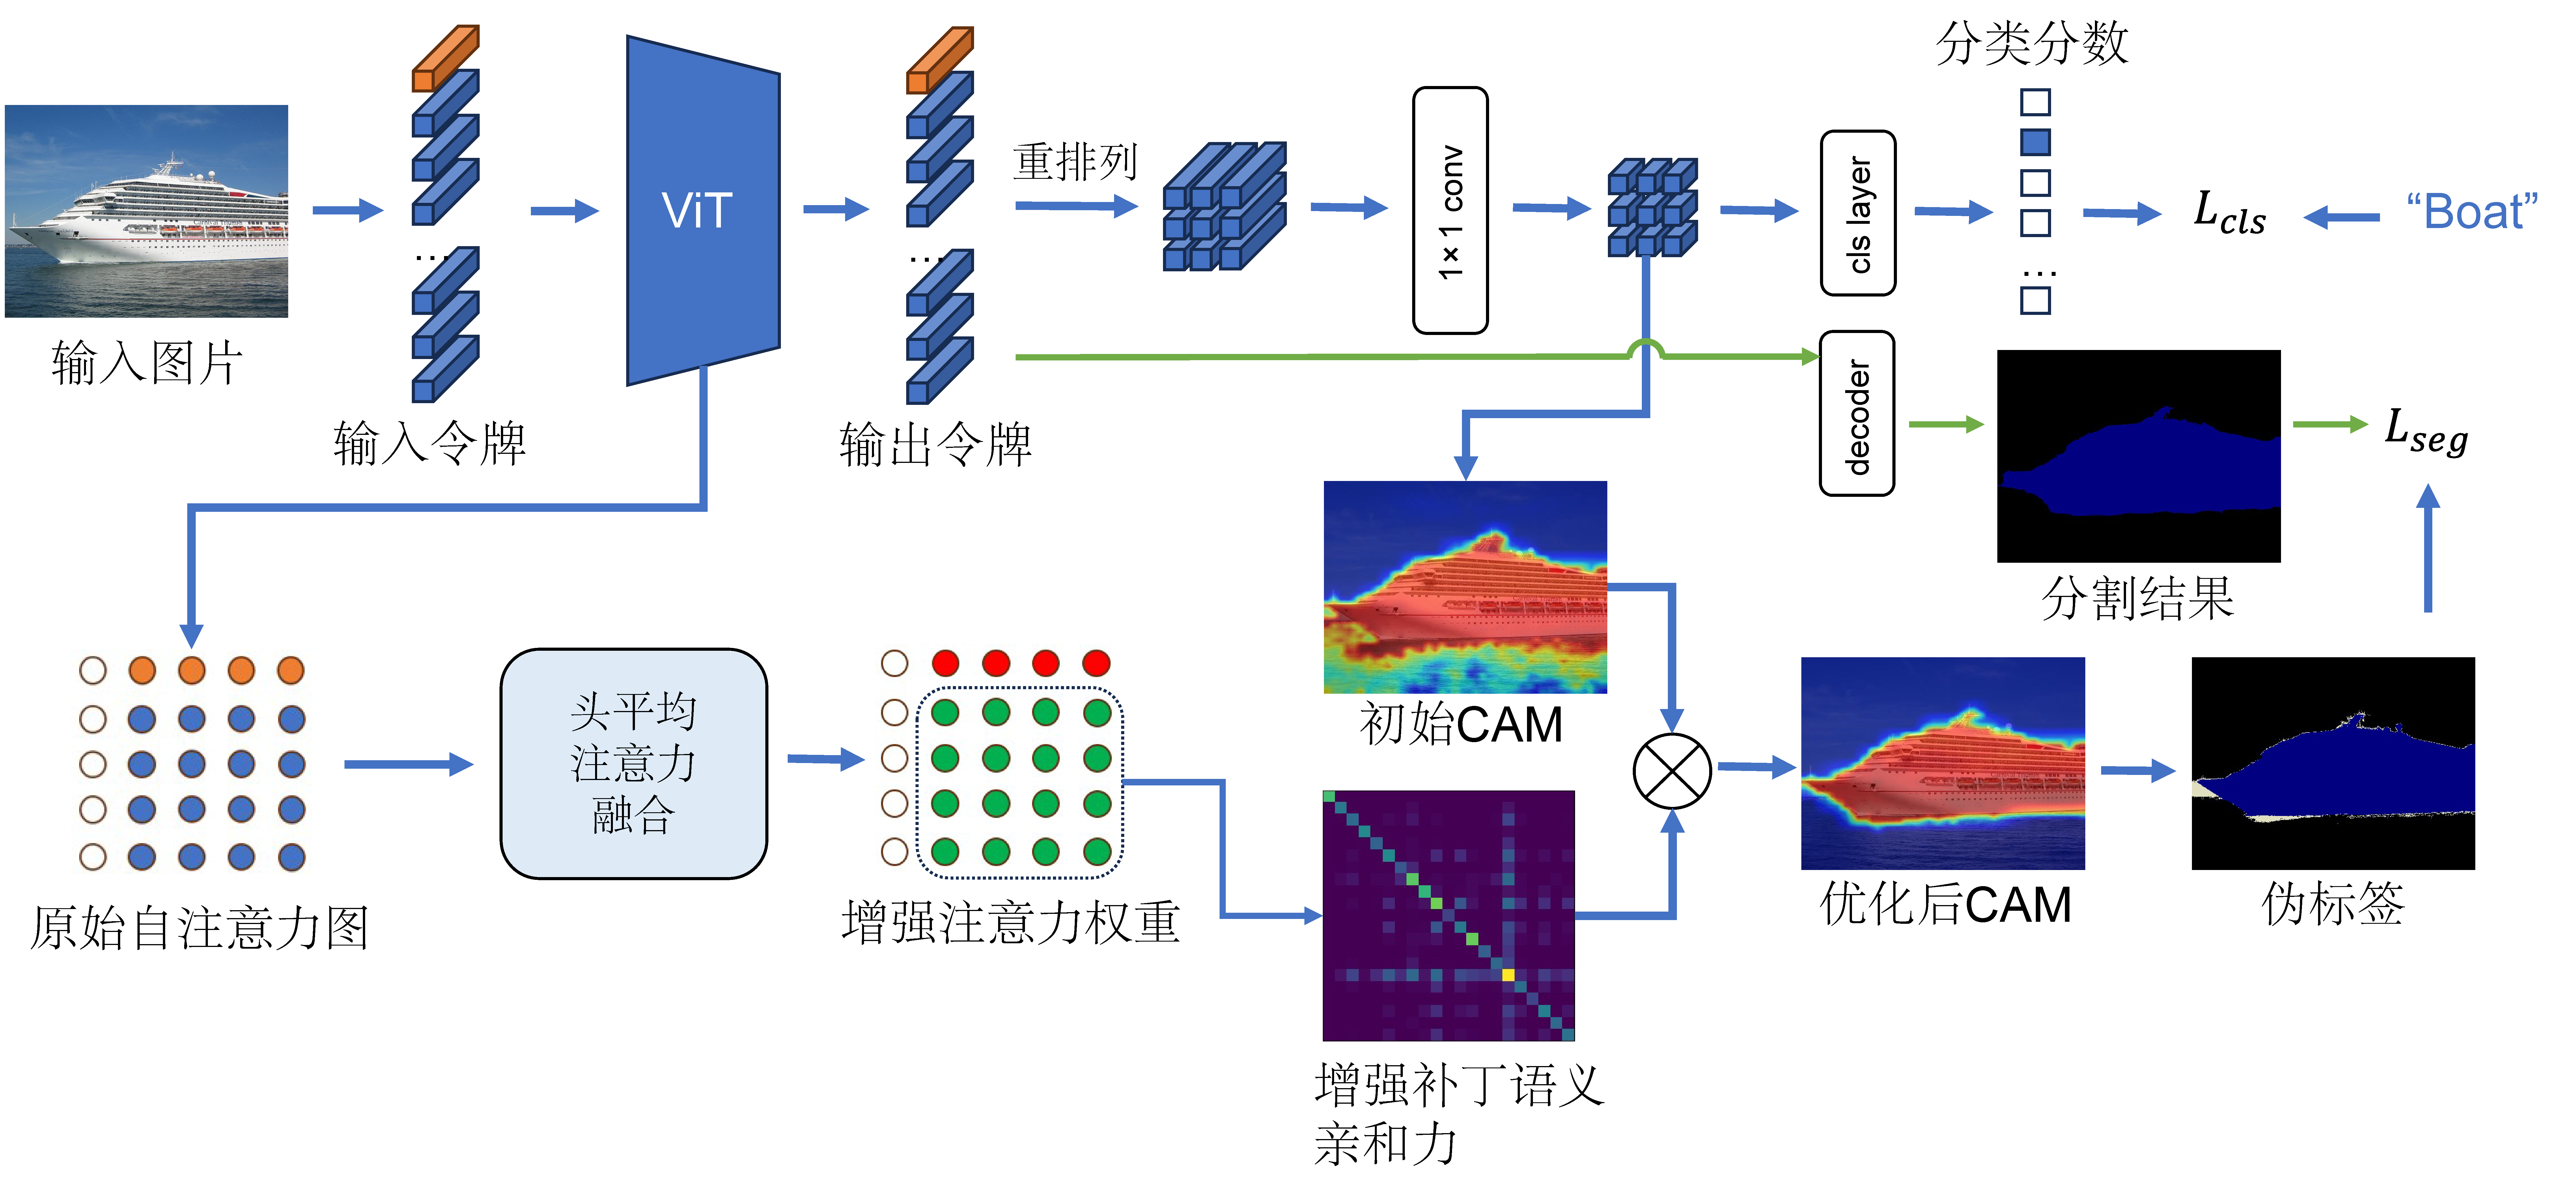
\includegraphics[width=6in]{fig/fig1.pdf}}
%     \begin{CJK*}{UTF8}{fs}
%         \caption{SS-EPA整体框架。SS-EPA首先将输入图像分成多个补丁,每个补丁线性转换成补丁令牌,并连接一个类别令牌。ViT输出令牌一方面经过重拍列和$1\times 1$卷积生成初始CAM,并由分类层输出分类分数。另一方面经过分割decoder生成语义分割结果。然后从ViT中提取多头自注意力图,并通过HAAF模块进行增强,获取增强补丁语义亲和力。最后通过增强补丁语义亲和力对初始CAM进行优化,并生成伪标签用于监督分割任务。}\label{fig1}
%     \end{CJK*}
% \end{figure*}

\vspace{2mm}

\begin{CJK*}{UTF8}{zhhei}
    \subsection{SS-EPA框架}\label{section3.2}
\end{CJK*}





SS-EPA首先将输入图片拆分为 $N\times N$ 个补丁,并通过线性转换为补丁令牌序列 $T_{\text{patch}}\in R^{N^2\times D}$,其中D是嵌入维度。
生成一个维度同样为D的类令牌 $T_{\text{cls}}\in R^{1\times D}$,将类令牌与补丁令牌链接,并添加位置编码构成ViT编码器的输入令牌序列 $T_{\text{input}}\in R^{(1+N^2)\times D}$。
ViT backbone具有$K$个Transformer编码层,每个编码层包含一个多头自注意力和一个多层感知机,以及分别用于两个子层前的层归一化。
ViT编码器接收输入令牌序列$T_{\text{input}}^i,i=(1,2,…,K)$,并输出令牌序列$T_{\text{out}}^i\in R^{(1+N^2)\times D},i=(1,2,…,K)$。
最后一层Transformer编码层的输出令牌序列$T_{\text{out}}^K\in R^{(1+N^2)\times D}$,去除类令牌对应维度并重排列可得补丁令牌序列$T_{\text{out\_patch}}\in R^{N\times N\times D}$,并执行$1\times 1$卷积操作将令牌维度变为物体类别数量,公式如下:

\begin{equation}
    \text{CAM}=\text{conv}_{1\times 1} (T_\text{out\_patch})
\end{equation}
其中,$\text{conv}_{1\times 1}$的输入通道为D,输出通道为物体类别数$C$,卷积核大小为$1\times 1$。通过上式可获得来自补丁令牌的初始类激活图$\text{CAM}\in R^{N\times N\times C}$。参照\cite{13ru2022learning}的方法,通过一个全局最大池化层(Global Max Pooling)来聚合补丁令牌$T_{\text{out\_patch}}$信息,然后通过全连接层来计算分类分数cls\_score,分类损失函数使用多标签软边距损失(Multi Label Soft Margin Loss)作为损失函数$L_{cls}$,公式如下:
\begin{equation}
    \begin{aligned}
        L_\text{cls}(x,y) = - \frac{1}{C}&\sum_{i=1}^C [y\log(\sigma (x)) \\
        &+(1-y)\log(1-\sigma (x))]
    \end{aligned}
\end{equation}
其中$x$,$y$分别是模型预测分数与真值标签,$\sigma(x)$表示Sigmoid函数的输出,即:
\begin{equation}
    \sigma(x) = \frac{1}{1+e^{-x}}
\end{equation}

ViT backbone使用的是标准的 Transformer 多头自注意力,首先将输入令牌归一化,并通过全连接层将其转换为一个查询$Q\in R^{(1+N^2)\times D}$和一组键值$K\in R^{(1+N^2)\times D}$、$V\times R^{(1+N^2)\times D}$,注意力计算采用\cite{14vaswani2017attention}中的缩放点积注意力(Scaled Dot-Product Attention),计算公式如下:

\begin{equation}
    \text{Attn}(Q,K,V)=\left(\text{Softmax}\frac{QK^T}{\sqrt{D}}\right)V
\end{equation}
从中可以提取多头自注意力图$A_{map}=QK^T$,其中$A_{\text{map}}^i\in R^{H\times (1+N^2)\times (1+N^2)} ,i=1,\cdots,K$,$H$为多头自注意力头的个数。此操作不会带来任何额外的计算资源消耗,因为多头自注意力权重是Transformer在计算时产生的副产物。然后在第$0$个维度上进行concatenate操作将$K$层注意力图串联起来,获得全局注意力张量$A\in R^{K\times H\times (1+N^2)\times (1+N^2)}$,该注意力张量十分庞大,在\ref{section3.3_HAAF}节中将讨论如何减小计算资源占用。

% \begin{figure*}[htbp]
%     \centerline{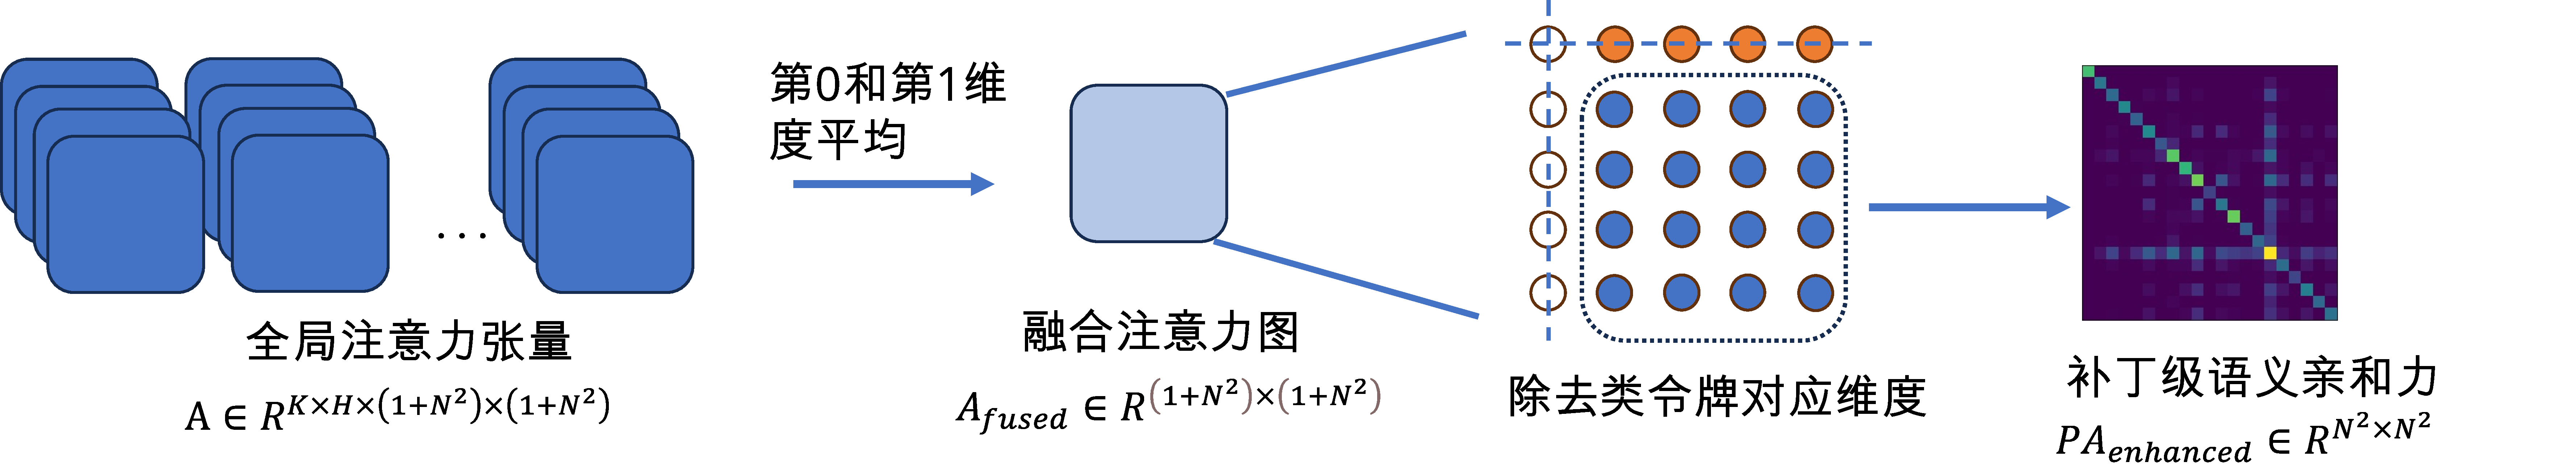
\includegraphics[width=6in]{fig/fig2.pdf}}
%     \begin{CJK*}{UTF8}{fs}
%         \caption{补丁语义亲和力获取流程图}\label{fig2}
%     \end{CJK*}
% \end{figure*}

全局注意力张量$A$中蕴含了补丁语义亲和力信息,将注意力图$A$在第$0$和第$1$个维度上进行平均来聚合来自不同层和不同头的注意力信息,得到$A_{\text{fused}}\in R^{(1+N^2)\times (1+N^2)}$,除去其中类令牌对应的维度,如图\ref{fig2}所示,剩下的注意力权重可作为补丁级语义亲和力$\text{PatchAffinity}\in R^{N^2 \times N^2}$。由于从补丁令牌生成的初始类激活图CAM存在大量噪声与错误,所以需要补丁级语义亲和力对其进行优化,优化公式如下:

\begin{equation}
    \text{CAM}_{\text{refined}}=\text{PatchAffinity}\times \text{CAM}
\end{equation}

通过上式可获得通过原始补丁语义亲和力优化后的类激活图$\text{CAM}_\text{refined}\in R^{N\times N\times C}$,相比初始CAM对目标的覆盖性更好,错误激活区域更少,且可以激活更多目标区域。


\vspace{2mm}


\begin{CJK*}{UTF8}{zhhei}
    \subsection{头平均注意力融合增强模块(HAAF)}
    \label{section3.3_HAAF}
\end{CJK*}

鉴于 Transformer 中不同深度的层的多头自注意力可能关注不同部分,如浅层更关注局部结构、纹理颜色等,深层能捕获更广泛和抽象的视觉语义信息,所以不能简单地将来自不同层的多头自注意力平均来聚合语义信息。
且一个标准ViT backbone(vit\_base\_patch16\_224)的多头自注意力图十分庞大(batchsize为2时,显存占用超过12GB),对计算资源要求较高。
本文提出头平均注意力融合增强模块(HAAF)来解决上述问题,如图\ref{fig3}所示。

\begin{figure}[htbp]
    \centerline{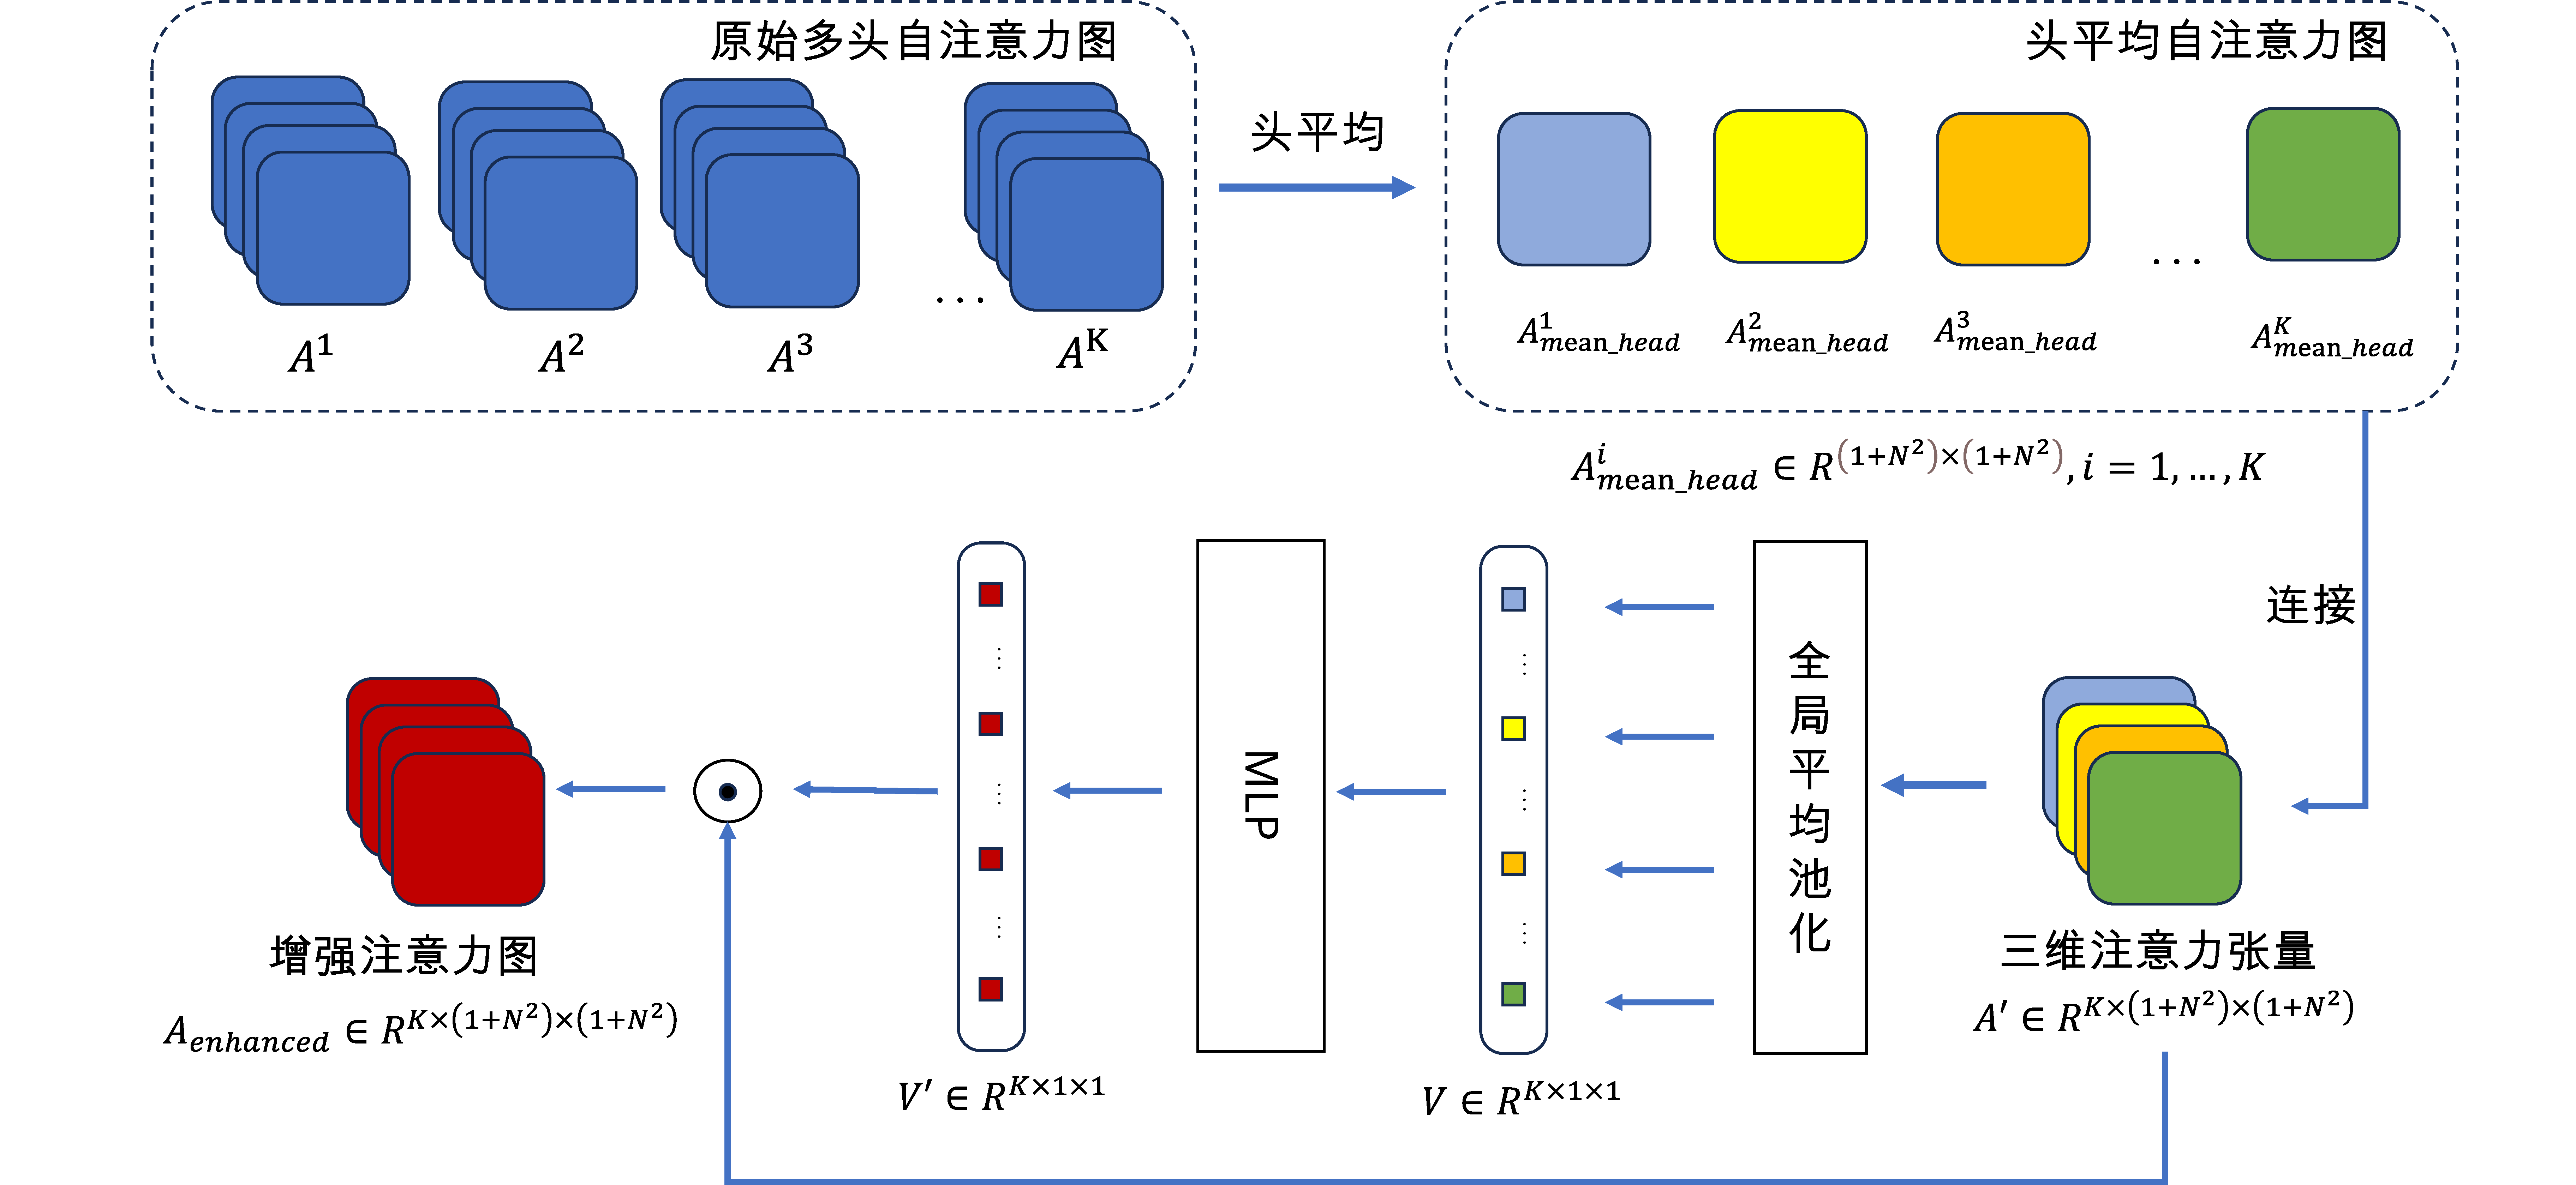
\includegraphics[width=3.15in]{fig/fig3.pdf}}
    \begin{CJK*}{UTF8}{fs}
        \caption{HAAF结构图}\label{fig3}
    \end{CJK*}
\end{figure}

\begin{figure*}[t]
    \centerline{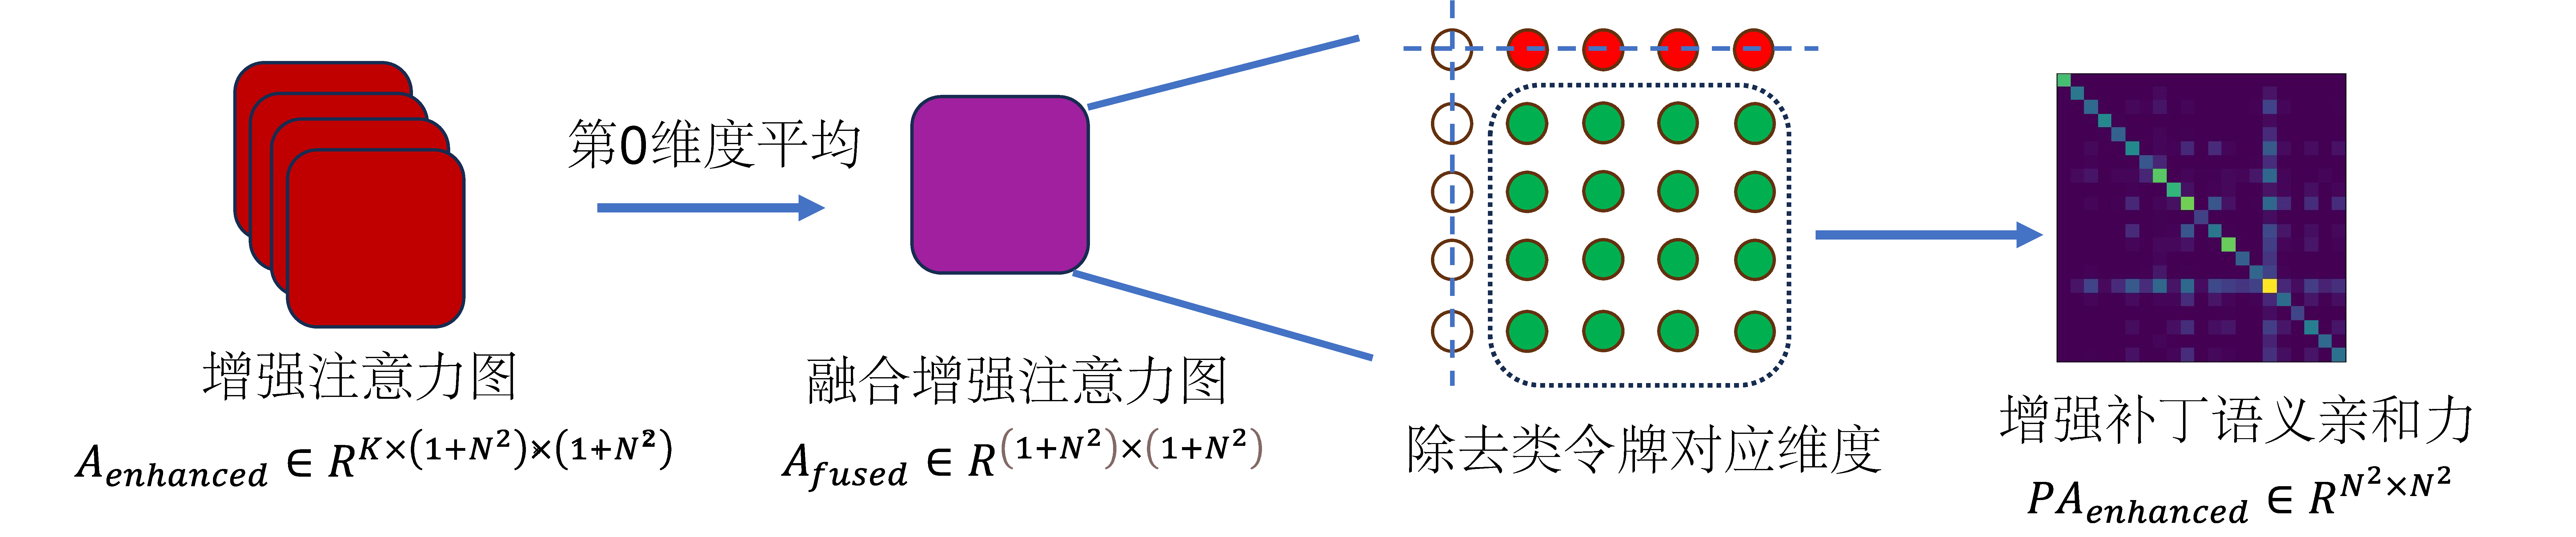
\includegraphics[width=6in]{fig/fig4.pdf}}
    \begin{CJK*}{UTF8}{fs}
        \caption{增强补丁语义亲和力获取流程图}\label{fig4}
    \end{CJK*}
\end{figure*}

对于\ref{section3.2}节中从backbone中提取的多头自注意力图$A_\text{map}^i\in R^{H\times (1+N^2)\times (1+N^2)},i=1,…,K$,HAAF首先采用头平均操作去除维度$H$,有助于去除冗余信息并减少$H$倍的显存占用,得到$A_\text{mean\_head}^i\in R^{(1+N^2)\times (1+N^2)},i=1,…,K$。
然后在第$0$个维度上进行concatenate操作将$K$层注意力图串联起来,获得全局注意力张量$A'\in R^(K\times (1+N^2)\times (1+N^2) )$。全局平均池化通过平滑特征表示和增强泛化能力,相较于全局最大池化,在减少噪声和防止过拟合方面更具优势。
所以本文通过全局平均池化聚合K层注意力图的全局特征,得到聚合后的长度为$K$的特征向量$V\in R^{K\times 1\times 1}$,并将特征向量输入多层感知机中相互作用,提取更复杂的特征相互关系,多层感知机输出相同形状的特征向量$V'\in R^(K\times 1\times 1)$。获得多层感知机输出的特征向量$V'$后,将全局注意力张量$A'$与特征向量$V'$结合,公式如下:
\begin{equation}
    A'_\text{enhanced} = A' \odot V'
\end{equation}
其中$\odot$表示逐元素相乘符号。
通过上式可获得充分考虑了不同层注意力重要性的增强注意力图$A_\text{enhanced}'\in R^{K\times (1+N^2)\times (1+N^2)}$。经过头平均后的注意力图更加稳定,不易受到单个注意力头学习偏差的影响。



% \begin{figure*}[htbp]
%     \centerline{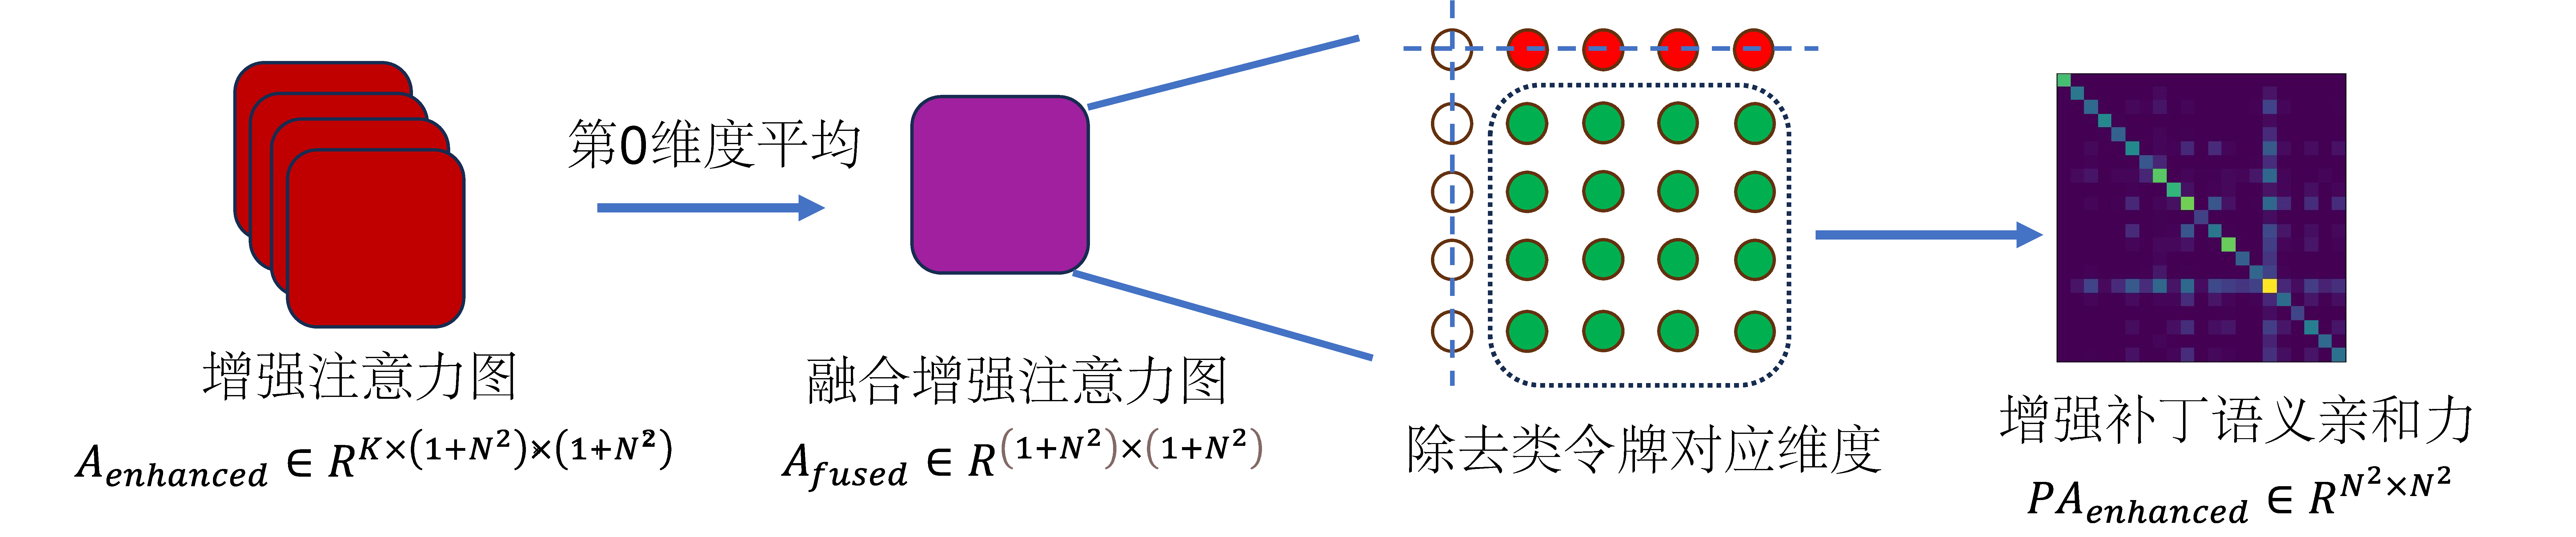
\includegraphics[width=6in]{fig/fig4.pdf}}
%     \begin{CJK*}{UTF8}{fs}
%         \caption{增强补丁语义亲和力获取流程图}\label{fig4}
%     \end{CJK*}
% \end{figure*}

图\ref{fig4}展示了不同层增强注意力图的融合过程,对增强注意力图$A_\text{enhanced}'$在第$0$个维度$K$上进行平均操作,可得到融合增强注意力$A_\text{fused}'\in R^{(1+N^2)\times (1+N^2)}$。
除去其中类令牌对应的维度,剩下的增强注意力权重可作为增强后的补丁级语义亲和力$\text{PA}_\text{enhanced}\in R^{N^2\times N^2}$,如图\ref{fig4}所示。通过HAAF增强后的补丁语义亲和力$\text{PA}_\text{enhanced}$相比增强前减少了噪声与错误,并且充分考虑了不同层注意力的重要性。通过特征向量$V'$对每层注意力进行加权。最后利用$\text{PA}_\text{enhanced}$对CAM优化,过程与3.2节介绍的CAM优化过程类似,优化公式如下:

\begin{equation}
\text{CAM}'_\text{refined} = \text{PA}_\text{enhanced} \times CAM
\end{equation}
其中$\text{CAM}$是来自补丁令牌的初始类激活图$\text{CAM}\in R^{N\times N\times C}$,通过上式可获得通过增强补丁语义亲和力优化后的类激活图$\text{CAM}_\text{refined}'\in R^(N\times N\times C)$。$\text{CAM}_\text{refined}'$相比直接利用语义亲和力优化的$\text{CAM}_\text{refined}$,拥有更全面的激活区域和更精细的对象边界,且有更高的鲁棒性。

\vspace{2mm}
\begin{CJK*}{UTF8}{zhhei}
    \subsection{模型训练与损失函数}
\end{CJK*}

如图\ref{fig1}所示,使用多标签软边缘损失作为分类损失$L_\text{cls}$,使用交叉熵损失作为分割损失$L_\text{seg}$。参照基线方法ToCo[3],本文使用了辅助分类损失$L_\text{m\_cls}$,以及令牌对比损失$L_\text{ptc}$和$L_\text{ctc}$。此外,为了进一步提高性能,还按照先前的方法\cite{13ru2022learning,15tang2018regularized,16zhang2021dynamic,17zhang2020reliability},采用了正则化损失$L_\text{reg}$,所以SS-EPA的损失最终定义如下:

\begin{equation}
    \begin{aligned}
        L=&L_\text{cls}+\lambda_1 L_\text{seg}+\lambda_2 L_\text{m\_cls}\\
        &+\lambda_3 L_\text{ptc}+ \lambda_4 L_\text{ctc}+ \lambda_5 L_\text{reg}
    \label{equation_8}
    \end{aligned}
\end{equation}
其中,超参数$\lambda_i,i=1,2,\cdots,5$用于平衡不同损失的权重。
